\documentclass[10pt]{article}
\usepackage[utf8]{inputenc}
\usepackage[T1]{fontenc}
\usepackage{amsmath}
\usepackage{amsfonts}
\usepackage{amssymb}
\usepackage[version=4]{mhchem}
\usepackage{stmaryrd}
\usepackage{graphicx}
\usepackage[export]{adjustbox}
\graphicspath{ {./images/} }

\begin{document}
Note 1: You must explain all your calculations clearly to get full credit.

Note 2: This assessment will be graded out of 40 marks. $90 \%$ of the grade for this coursework (36/40) will be assigned for a correct, well-argued calculation. Another $10 \%(4 / 40)$ will be awarded at the grader's discretion for clarity and presentation of your solution.

Note 3: Due by midday on Monday March 13th 2023. Please submit via the Turnitin dropbox link provided in Blackboard.

Part I: For any integer $n \geq 0$ define

$$
I_{+}(n) \equiv \int_{0}^{1} e^{y} \sin (n \pi y) d y, \quad I_{-}(n) \equiv \int_{0}^{1} e^{-y} \sin (n \pi y) d y .
$$

(i) Calculate these two integrals explicitly.

(ii) Use the result of part (i) to find the Fourier sine series of both $\sinh y$ and cosh $y$ over the interval $[0,1]$ (you should use ideas from the "Calculus and Applications" course).

Part II: Consider the electric circuit shown in the Figure where the vertical edges have conductance $c$ and the horizontal edges have conductance $d$. Node $2 \mathrm{~N}+1$ is set to unit voltage, while nodes 0 and $\mathrm{N}+1$ to $2 \mathrm{~N}$ are grounded (set to zero voltage). Kirchhoff's current law holds at nodes 1 to $\mathrm{N}$. Let $\hat{\mathbf{x}}$ denote the voltages at nodes 1 to $\mathrm{N}$. The nodes should be ordered as follows: $1,2, \ldots, 2 \mathrm{~N}-1,2 \mathrm{~N}$, $0,2 \mathrm{~N}+1$.

(a) Show that the conductance-weighted Laplacian matrix is

$$
\mathbf{K}=\left(\begin{array}{ccc}
c \mathbf{K}_{N}+d \mathbf{I}_{N} & -d \mathbf{I}_{N} & -c \mathbf{P} \\
-d \mathbf{I}_{N} & d \mathbf{I}_{N} & \mathbf{0} \\
-c \mathbf{P}^{T} & \mathbf{0} & c \mathbf{I}_{2}
\end{array}\right),
$$

where $\mathbf{I}_{j}$ denotes the $j$-by- $j$ identity matrix and $\mathbf{K}_{N}$ is the $N$-by- $N$ matrix familiar from lectures. You should find the $N$-by-2 matrix $\mathbf{P}$.

(b) Let $\left\{\boldsymbol{\Phi}_{\mathbf{j}} \mid j=1, \ldots, N\right\}$ and $\left\{\lambda_{j} \mid j=1, \ldots, N\right\}$ denote the orthonormal eigenvectors and corresponding eigenvalues of $\mathbf{K}_{N}$. By writing

$$
\hat{\mathbf{x}}=\sum_{j=1}^{N} a_{j}(\mu) \boldsymbol{\Phi}_{j}, \quad \mu=\frac{d}{c}
$$

find the coefficients $\left\{a_{j}(\mu) \mid j=1, \ldots, N\right\}$.

\begin{center}
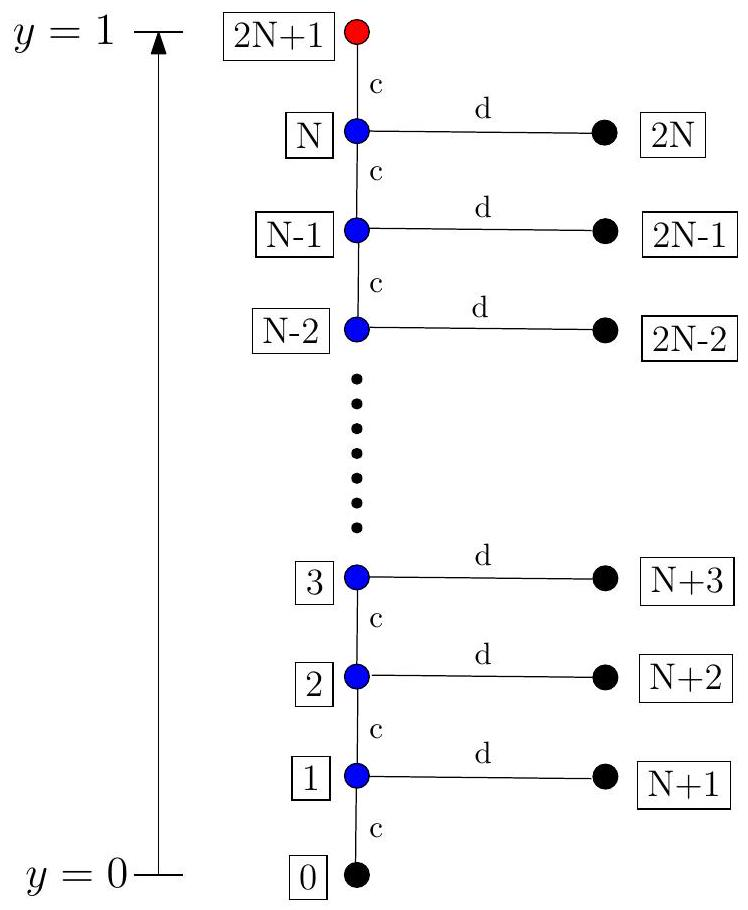
\includegraphics[max width=\textwidth]{2023_03_08_5758588d6e703b32009fg-2}
\end{center}

(c) Show that the $n$-th element of $\hat{\mathbf{x}}$ can also be written as

$$
\frac{\lambda_{+}(\mu)^{n}-\lambda_{-}(\mu)^{n}}{\lambda_{+}(\mu)^{N+1}-\lambda_{-}(\mu)^{N+1}}, \quad n=1, \ldots, N,
$$

for suitable choices of the parameters $\lambda_{ \pm}(\mu)$.

(d) The uniqueness theorem for harmonic potentials discussed in lectures has an analogous version when the conductances are not all equal. Use this fact to establish a discrete identity involving your answers to parts (b) and (c).

(e) Now pick $\mu$ to be given by

$$
\mu=\frac{1}{(N+1)^{2}}
$$

and introduce the new variable

$$
y=\frac{n}{(N+1)}
$$

Find the limit of both left- and right-hand sides of the discrete identity you found in part (d) as $N \rightarrow \infty$ with $y$ taken to be fixed.

\section{THE END}

\end{document}